% =============================================================================
% PART II: PROGRESS AFTER THE MID-REVIEW
% =============================================================================

% -----------------------------------------------------------------------------
\section{Overview of the Second Phase}
\label{sec:phase2}
% -----------------------------------------------------------------------------

After the mid-review we took a step back and asked a simple question: \emph{are the designs from Part~\ref{part:mid} correct when a real operating system runs on top of them?} Every result in Part~\ref{part:mid} came from SE mode, where \texttt{gem5} emulates the operating system, and from small single-process microbenchmarks. In SE mode many events that matter for a TLB never happen. There are no context switches with a real CR3 write, no \texttt{INVLPG} instructions when the kernel unmaps a page, no process IDs (PCIDs) in use, and no kernel code sharing the TLB with the program.

So the second phase focused on depth instead of adding new mechanisms from the mid-review's next-steps list. It had five stages, shown in Figure~\ref{fig:phase2_flow}:
\begin{enumerate}
    \item An implementation audit of every design.
    \item Correctness fixes for every design, kept as separate \texttt{.fixed} source files.
    \item Verification of every design against a translation oracle in SE mode.
    \item Full-system evaluation on an Ubuntu 24.04 guest running all 43 SPEC CPU2017 benchmarks, for every design.
    \item Performance study on TLB-intensive workloads, including the graph and key-value store benchmarks suggested by the instructor, with CoLT-FA as the main focus.
\end{enumerate}

\begin{figure}[htbp]
\centering
\begin{tikzpicture}[
  node distance=0.45cm and 0.5cm,
  box/.style={draw, rounded corners, fill=#1, minimum width=2.45cm, minimum height=1.25cm, align=center, font=\scriptsize},
  box/.default=blue!8,
  arr/.style={-{Stealth[length=2mm]}, thick}]
\node[box=gray!12] (a) {\textbf{1. Audit}\\read every design,\\list gaps};
\node[box=orange!12, right=of a] (b) {\textbf{2. Fix}\\one \texttt{.fixed}\\file per design};
\node[box=green!12, right=of b] (c) {\textbf{3. Verify (SE)}\\oracle checker,\\stress tests};
\node[box=blue!10, right=of c] (d) {\textbf{4. Full system}\\43 SPEC benchmarks\\x 6 designs};
\node[box=red!10, right=of d] (e) {\textbf{5. Performance}\\GAPBS, memcached,\\XSBench, SPEC ref};
\draw[arr] (a) -- (b); \draw[arr] (b) -- (c); \draw[arr] (c) -- (d); \draw[arr] (d) -- (e);
\node[below=0.35cm of c, font=\scriptsize, text width=11cm, align=center] {CoLT-FA joined at stage 2 as the sixth design and was carried through stages 3 to 5};
\end{tikzpicture}
\caption{Stages of the second phase.}
\label{fig:phase2_flow}
\end{figure}

Table~\ref{tab:designs} lists the six designs evaluated in this phase. All of them keep the 64-entry L1 TLB and the 128-set, 4-way L2 TLB with XOR-7 indexing from Part~\ref{part:mid}, unless a design changes the L2 itself.

\begin{table}[htbp]
\centering
\small
\caption{The six L2 TLB designs evaluated in the second phase.}
\label{tab:designs}
\begin{tabularx}{\textwidth}{l l X}
\toprule
\textbf{Design} & \textbf{Source files} & \textbf{What it does} \\
\midrule
Inclusive & \texttt{tlb.\{cc,hh\}.inc.fixed} & Every L1 entry also lives in the L2 (Section~3.2.1). \\
Exclusive & \texttt{tlb.\{cc,hh\}.excl.fixed} & A translation lives in only one level; L2 hits are promoted, L1 victims spill to L2. \\
NINE & \texttt{tlb.\{cc,hh\}.nine.fixed} & L1 and L2 are filled independently. \\
Agile / NaiveFP & \texttt{tlb.\{cc,hh\}.agile.fixed} & NINE plus a prefetcher that installs neighbouring translations, now with runtime parameters. \\
Perforated Pages & \texttt{tlb.\{cc,hh\}.perf.fixed} & L2 entries cover 2MB regions with a validity bitmap and a coarse filter (Section~6). \\
CoLT-FA & \texttt{tlb.\{cc,hh\}.colt.fixed} & NINE plus an 8-entry fully associative buffer of coalesced runs of up to 8 pages (Section~\ref{sec:colt_fs}). \\
\bottomrule
\end{tabularx}
\end{table}

% -----------------------------------------------------------------------------
\section{Implementation Audit}
\label{sec:audit}
% -----------------------------------------------------------------------------

The first task was a line-by-line audit of every TLB variant from Part~\ref{part:mid} (recorded in \texttt{TLB\_IMPLEMENTATION\_AUDIT.md}). The audit found problems in how the designs were built and tested, and also in what the code did when an operating system is present. Table~\ref{tab:audit} summarises the findings.

\begin{table}[htbp]
\centering
\small
\caption{Main findings of the implementation audit.}
\label{tab:audit}
\begin{tabularx}{\textwidth}{l X X}
\toprule
\textbf{\#} & \textbf{Finding} & \textbf{Why it matters} \\
\midrule
1 & The policy files were snapshots (for example \texttt{tlb.cc.inclusive.sa}). Only \texttt{tlb.cc} is compiled, so a design was only active if its snapshot was copied over \texttt{tlb.cc} before the build. & It was easy to measure a different design from the one intended. Each design now has its own build. \\
2 & The L2 was not invalidated when the kernel unmaps a page (\texttt{demapPage}) or switches address space (\texttt{flushNonGlobal} on a CR3 write) in several designs. & A stale L2 entry could hand out an old physical address after the page was freed or remapped. \\
3 & The L2 removal function matched entries by virtual address only and ignored the PCID stored in the low 12 bits of the key. & An unmap in one process could remove another process's entry, or miss its own. \\
4 & \texttt{serialize}/\texttt{unserialize} saved only the L1 array. & After a checkpoint restore the L2 state was silently lost. \\
5 & The Perforated Pages and Agile prefetch code were not integrated into a buildable, testable form, and the Agile prefetcher cited the wrong paper. & Results could not be reproduced. The citation was corrected to Vavouliotis et al.~\cite{vavouliotis2021agile}. \\
6 & No test compared the TLB's answer with the true page table. Results were raw miss counts. & A design that returns wrong translations can still show fewer misses. \\
\bottomrule
\end{tabularx}
\end{table}

An important point from the audit is that findings 2 and 3 cannot be triggered in SE mode. In SE mode \texttt{gem5} never calls \texttt{demapPage}, because it is only reached from full-system code paths (the page fault handler and the \texttt{INVLPG} instruction), and it always uses PCID 0. This is why the second phase had to move to full-system simulation (Section~\ref{sec:fs_method}).

% -----------------------------------------------------------------------------
\section{Correctness Fixes for Each Design}
\label{sec:fixes}
% -----------------------------------------------------------------------------

Each design was fixed in a new source file (\texttt{tlb.cc.<design>.fixed} and \texttt{tlb.hh.<design>.fixed}), so the original snapshots stay unchanged for comparison. The fixes common to all designs are listed first, followed by the design-specific ones.

\subsection{Fixes Common to All Designs}
\begin{itemize}
    \item \textbf{L2 invalidation on unmap}: \texttt{demapPage(va, asn)} now also removes the matching L2 entry.
    \item \textbf{L2 invalidation on address-space switch}: \texttt{flushNonGlobal()} now clears every non-global L2 entry, as it already did for the L1.
    \item \textbf{PCID-aware removal}: \texttt{l2\_remove} now builds the same \texttt{concAddrPcid(vpn, pcid)} key that \texttt{l2\_insert} uses, so only the translation of the right address space is removed.
    \item \textbf{Checkpointing}: the L2 contents are saved and restored together with the L1 (Perforated Pages clears the L2 on restore instead).
    \item \textbf{Statistics}: new counters for L2 hits, insertions and evictions (\texttt{l2Hits}, \texttt{l2Insertions}, \texttt{l2Evictions}).
    \item \textbf{Runtime parameters}: L2 geometry, hash function and replacement policy can be chosen with environment variables, so one binary can be used for a whole parameter sweep without rebuilding.
\end{itemize}

\subsection{Design-Specific Fixes}

\paragraph{Inclusive.} Four issues were fixed (Table~\ref{tab:inc_bugs}). While fixing the checkpoint code we also found that \texttt{gem5}'s checkpoint format is positional: a value written after a group of entries is read back as part of that group. The first two attempts at the fix failed on restore for this reason, and the third attempt placed all L2 values in their own section.

\begin{table}[htbp]
\centering
\small
\caption{Inclusive design: issues found and fixed.}
\label{tab:inc_bugs}
\begin{tabularx}{\textwidth}{l X X}
\toprule
\textbf{\#} & \textbf{Issue} & \textbf{Fix} \\
\midrule
1 & \texttt{l2\_remove(va)} ignored the PCID. & Removal uses the full \texttt{(va, pcid)} key. \\
2 & Checkpoints held only the L1 (a checkpoint taken after a 2,048-page run had 64 L1 entries and no L2 keys). & L2 sets and entries are serialized. \\
3 & Checkpoint values placed after the entry list were read back in the wrong section. & L2 state written in its own section. \\
4 & L2 geometry, hash and replacement were compile-time constants. & Selectable at runtime (\texttt{TLB\_L2\_GEOM}, \texttt{TLB\_L2\_HASH}, \texttt{TLB\_L2\_REPL}, \texttt{TLB\_L1\_SIZE}). \\
\bottomrule
\end{tabularx}
\end{table}

\paragraph{Exclusive.} The exclusive policy requires that a translation is never in both levels at once. We added a checker for this rule. With several hardware threads sharing the TLB (SMT), promotion and eviction could leave duplicate translations: the checker recorded \textbf{391,950 duplicate violations in 1,368,154 checks} on the original code. After the fix the same run reports \textbf{0} violations. The PCID-aware removal and the L2 checkpointing were fixed as for the other designs.

\paragraph{NINE.} The same PCID and checkpoint issues were fixed. Since NINE has no inclusion rule to check, a \emph{staleness scan} was added instead: after every flush, unmap and checkpoint restore, every valid L1 and L2 entry is checked again against the page table. On the \texttt{remap} stress test the scan ran 30 times and found no stale entry.

\paragraph{Agile / NaiveFP.} Seven issues were fixed in the prefetching design (Table~\ref{tab:agile_bugs}). The prefetcher was also turned into a runtime-parameterised design (degree, direction, adaptive degree, throttling and priority are selected with \texttt{AGILE\_PF\_*} variables) with counters for issued, useful and unused prefetches.

\begin{table}[htbp]
\centering
\small
\caption{Agile / NaiveFP design: issues found and fixed.}
\label{tab:agile_bugs}
\begin{tabularx}{\textwidth}{l X}
\toprule
\textbf{\#} & \textbf{Issue} \\
\midrule
1 & \texttt{l2\_remove()} was declared in the header but never defined. \\
2 & \texttt{demapPage()} never touched the L2. \\
3 & \texttt{demapPage()} looked up the L1 with the raw address instead of the PCID-tagged key. \\
4 & \texttt{flushNonGlobal()} never touched the L2. \\
5 & Checkpoints never saved or restored the L2. \\
6 & No prefetch counters, so useful prefetches could not be told apart from wasted ones. \\
7 & In our own adaptive-degree code, the degree was reset on every window boundary, even after a successful window (found and fixed during the campaign). \\
\bottomrule
\end{tabularx}
\end{table}

\paragraph{Perforated Pages.} Six issues were fixed (Table~\ref{tab:perf_bugs}). Issue 4 is the most serious: every L2 hit returned a translation with hard-coded permissions (user access allowed, execution allowed), so in full-system mode a user program could have been given access to a kernel page.

\begin{table}[htbp]
\centering
\small
\caption{Perforated Pages design: issues found and fixed.}
\label{tab:perf_bugs}
\begin{tabularx}{\textwidth}{l X X}
\toprule
\textbf{\#} & \textbf{Issue} & \textbf{Fix} \\
\midrule
1 & \texttt{demapPage()} cleared only the L1, so the L2 kept a stale sub-page. & Also clears the sub-page in the L2 and updates its coarse filter. \\
2 & \texttt{flushNonGlobal()} cleared only the L1. & Also clears non-global L2 regions. \\
3 & L2 regions had no address-space tag. & A \texttt{pcid} field is part of the match. \\
4 & L2 hits were rebuilt with hard-coded \texttt{user=true}, \texttt{noExec=false}, \texttt{global=false}. & The real per-page permissions are stored and returned. \\
5 & On every SE miss, \texttt{l2\_insert()} was called twice for the same page. & The extra call was removed. \\
6 & Checkpoints never touched the L2. & The L2 is cleared on restore. \\
\bottomrule
\end{tabularx}
\end{table}

\paragraph{CoLT-FA.} CoLT-FA needed the most work and is described in its own section (Section~\ref{sec:colt_fs}).

% -----------------------------------------------------------------------------
\section{Verification Framework}
\label{sec:verif}
% -----------------------------------------------------------------------------

\subsection{Translation Oracle and Invariant Checkers}
To check correctness instead of only counting misses, we added an instrumentation layer to \texttt{tlb.cc}. It is applied by a script (\texttt{robustness/patches/apply\_checker*.py}) so that the same checker is used for every design:
\begin{itemize}
    \item \textbf{Translation oracle}: every time a translation finishes, the physical address given by the TLB is compared with the true one. In SE mode the true answer comes from the process page table. In full-system mode the checker does its own functional page walk of the guest page table every $N$-th translation ($N = 64$ by default, set with \texttt{TLBCHK\_FS\_PERIOD}).
    \item \textbf{Inclusion invariant} (Inclusive): every valid L1 entry must have a matching L2 entry.
    \item \textbf{Exclusivity invariant} (Exclusive): no translation may be valid in both levels.
    \item \textbf{Staleness scan} (NINE, CoLT-FA): after every flush, unmap and restore, every valid entry is re-checked against the page table.
\end{itemize}
Mismatches are counted in \texttt{stats.txt} (\texttt{chkOracleMismatch}, \texttt{chkOracleWalkFault}, \texttt{chkStaleL1}, \texttt{chkStaleL2}) and the first few are printed with details.

\subsection{Stress Tests}
Three test programs were written for the SE-mode matrix (\texttt{robustness/tests/}):
\begin{itemize}
    \item \texttt{tlbstress}: capacity, set-conflict, remap, protection change, huge page, TLB shootdown, multi-thread, multi-process, interrupt and shared-memory tests.
    \item \texttt{pf\_patterns}: nine access patterns (ascending, descending, strides 2/4/8/16, random, pointer chasing, hot/cold) over a chosen number of pages.
    \item \texttt{perf\_holes}: 2MB regions with different hole patterns (dense, edge, clustered, dispersed, one hole per 64 pages, sparse, churn) for Perforated Pages.
\end{itemize}
These were combined into a job matrix covering Atomic, Timing and O3 CPUs, single and multiple cores, multi-threaded and multi-programmed runs, SMT with 2 and 4 threads, and fork with shared memory. Every job was run on the design under test \emph{and} on stock \texttt{gem5}, so a failure that also happens on stock \texttt{gem5} can be separated from a failure of the design.

\subsection{Problems in the Test Harness}
Two harness problems were found and fixed while setting up SPEC CPU2017 in SE mode:
\begin{itemize}
    \item \texttt{gem5}'s SE configuration redirects any guest path under \texttt{/tmp} into its own output directory. Since the SPEC installation was under \texttt{/tmp}, SPEC could not find its own files. The installation was moved to \texttt{/var/tmp}.
    \item Some SPEC benchmarks take options that start with a dash (for example \texttt{-I./lib} for perlbench), which \texttt{se.py} tried to read as its own options. The job generator was changed to pass the options as a single argument.
\end{itemize}

% -----------------------------------------------------------------------------
\section{SE-Mode Verification Results}
\label{sec:se_results}
% -----------------------------------------------------------------------------

\subsection{Correctness Matrix}
Table~\ref{tab:se_matrix} gives the SE-mode results. \textbf{No design produced a single oracle mismatch.} Every failure in the matrix also fails, in the same way, on stock \texttt{gem5}: these are known limits of SE mode (\texttt{setitimer} not implemented, fork with \texttt{MAP\_SHARED} hanging past the timeout, and multi-process remap tests that see stale data on stock \texttt{gem5} too).

\begin{table}[htbp]
\centering
\small
\caption{SE-mode correctness results. "Same on stock" means every failing job also fails identically on unmodified \texttt{gem5}.}
\label{tab:se_matrix}
\begin{tabularx}{\textwidth}{l l l X}
\toprule
\textbf{Design} & \textbf{Matrix} & \textbf{Oracle mismatches} & \textbf{Notes} \\
\midrule
Inclusive & 94/120 (original), 47/54 (fixed) & 0 & 26 failures, all same on stock; 0 inclusion violations \\
Exclusive & 94/120 & 0 & all 26 failures same on stock; duplicate violations 391,950 $\rightarrow$ 0 \\
NINE & 94/120 (original), 47/57 (fixed) & 0 & 0 design-specific failures; staleness scan found 0 stale entries \\
Agile / NaiveFP & 20/24 tlbstress, 108/108 \texttt{pf\_patterns} & 0 & the 4 failures (shared memory) hang on stock too \\
Perforated Pages & 36/44 & 0 & the 8 non-passes identical on stock; 31 configurations swept \\
CoLT-FA & 36/36 & 0 & see Section~\ref{sec:colt_se} \\
\bottomrule
\end{tabularx}
\end{table}

\subsection{SPEC CPU2017 in SE Mode}
For the Inclusive design, all SPEC CPU2017 rate benchmarks that could be built were run with test inputs on the Atomic CPU, on both the fixed design and stock \texttt{gem5}, with the oracle and inclusion checker turned on. \textbf{All 31 SPEC invocations that could run passed, with 0 inclusion violations, 0 oracle mismatches and output identical to stock \texttt{gem5}.} The two that could not run (perlbench and omnetpp) failed on both builds because of the option problem described above.

\subsection{Design Parameter Sweeps}
Because the fixed designs take their parameters at runtime, each design was swept with a single binary. All variants kept 0 correctness errors. Tables~\ref{tab:sweep_inc} to~\ref{tab:sweep_perf} show selected rows.

\begin{table}[htbp]
\centering
\small
\caption{Inclusive design: selected variants (adversarial set-conflict benchmark, Atomic CPU). L2 hits and back-invalidations of the L1 caused by L2 evictions.}
\label{tab:sweep_inc}
\begin{tabular}{l c c c r r}
\toprule
\textbf{Variant} & \textbf{Geometry} & \textbf{Hash} & \textbf{Repl.} & \textbf{L2 hits} & \textbf{Back-inval.} \\
\midrule
Default & 128$\times$4 & XOR-7 & LRU & 0 & 3,130 \\
Geometry 64$\times$8 & 64$\times$8 & XOR-7 & LRU & 1,973 & 0 \\
Geometry 256$\times$2 & 256$\times$2 & XOR-7 & LRU & 1,925 & 20 \\
Fully associative & 1$\times$512 & XOR-7 & LRU & 1,973 & 0 \\
Modulo hash & 128$\times$4 & modulo & LRU & 1,973 & 0 \\
XOR-fold hash & 128$\times$4 & XOR-fold & LRU & 0 & 3,030 \\
Random replacement & 128$\times$4 & XOR-7 & random & 0 & 3,151 \\
\bottomrule
\end{tabular}
\end{table}

\begin{table}[htbp]
\centering
\small
\caption{Exclusive design: selected variants. TLB misses of the design against stock \texttt{gem5} (36,348 misses).}
\label{tab:sweep_excl}
\begin{tabular}{l l r r}
\toprule
\textbf{Variant} & \textbf{Setting} & \textbf{Misses} & \textbf{Change vs stock} \\
\midrule
Default & 128 sets, 4 ways, XOR-7, LRU, always spill & 9,063 & $-75.1\%$ \\
Sets 64 & \texttt{EXCL\_L2\_SETS=64} & 23,491 & $-35.4\%$ \\
Sets 256 & \texttt{EXCL\_L2\_SETS=256} & 5,891 & $-83.8\%$ \\
Ways 2 & \texttt{EXCL\_L2\_WAYS=2} & 26,658 & $-26.7\%$ \\
Modulo hash & \texttt{EXCL\_L2\_HASH=1} & 6,114 & $-83.2\%$ \\
Dirty-hot spill & \texttt{EXCL\_SPILL=dirty-hot} & 36,244 & $-0.3\%$ \\
No spill & \texttt{EXCL\_SPILL=never} & 36,348 & $0.0\%$ \\
Smaller L1 & \texttt{EXCL\_L1\_SIZE=32} & 9,260 & $-74.5\%$ \\
\bottomrule
\end{tabular}
\end{table}

\begin{table}[htbp]
\centering
\small
\caption{NINE design: selected variants (L1 misses and L2 hits on the same workload).}
\label{tab:sweep_nine}
\begin{tabular}{l l r r r}
\toprule
\textbf{Variant} & \textbf{Setting} & \textbf{L2 entries} & \textbf{L1 misses} & \textbf{L2 hits} \\
\midrule
Default & none & 512 & 48,727 & 2,624 \\
Sets 64 & \texttt{NINE\_L2\_SETS=64} & 256 & 50,587 & 764 \\
Sets 256 & \texttt{NINE\_L2\_SETS=256} & 1,024 & 41,763 & 9,588 \\
Ways 2 & \texttt{NINE\_L2\_WAYS=2} & 256 & 50,576 & 775 \\
Ways 8 & \texttt{NINE\_L2\_WAYS=8} & 1,024 & 42,395 & 8,956 \\
Low-bits hash & \texttt{NINE\_L2\_HASH=1} & 512 & 48,003 & 3,348 \\
Random replacement & \texttt{NINE\_L2\_REPL=2} & 512 & 47,832 & 3,519 \\
\bottomrule
\end{tabular}
\end{table}

\noindent For NINE, doubling the total L2 capacity (more sets or more ways) roughly doubled the L2 hit rate, while the hash and replacement choice made a smaller difference at a fixed capacity.

\begin{table}[htbp]
\centering
\small
\caption{Agile prefetcher: selected variants (2,048 pages, 3 passes). Walks, issued prefetches, useful prefetches, and prefetches evicted unused (pollution).}
\label{tab:sweep_agile}
\begin{tabular}{l l r r r r}
\toprule
\textbf{Pattern} & \textbf{Variant} & \textbf{Walks} & \textbf{Issued} & \textbf{Useful} & \textbf{Unused} \\
\midrule
ascending & degree 1 & 4,919 & 20,041 & 5,436 & 52 \\
ascending & degree 4 & 4,324 & 70,308 & 6,031 & 172 \\
ascending & degree 8 & 4,224 & 136,584 & 6,131 & 236 \\
ascending & adaptive (exp) & 4,238 & 21,490 & 6,117 & 164 \\
ascending & degree 4, wrong direction & 10,287 & 263,392 & 68 & 177 \\
random & degree 1 & 9,054 & 48,986 & 1,305 & 32,430 \\
random & degree 8 & 8,767 & 422,793 & 1,601 & 289,525 \\
\bottomrule
\end{tabular}
\end{table}

\noindent For the Agile prefetcher, the adaptive degree reached almost the same number of walks as a fixed degree of 8 on the ascending pattern (4,238 against 4,224) while issuing about one sixth of the prefetches (21,490 against 136,584). On the random pattern most prefetches were never used.

\begin{table}[htbp]
\centering
\small
\caption{Perforated Pages: selected variants out of 31 (total L1 misses, one knob changed at a time).}
\label{tab:sweep_perf}
\begin{tabular}{l l r r}
\toprule
\textbf{Variant} & \textbf{Setting} & \textbf{L1 misses} & \textbf{vs baseline} \\
\midrule
Baseline & 128 sets, 4 ways, 8 chunks, prefetch 8, LRU & 149,703 & -- \\
All four fixes reverted & \texttt{PERF\_FIX\_*=0} & 149,703 & $+0.0\%$ \\
16 sets, 1 way & \texttt{PERF\_L2\_SETS=16 PERF\_L2\_WAYS=1} & 159,810 & $+6.8\%$ \\
1 set, 1 way & \texttt{PERF\_L2\_SETS=1 PERF\_L2\_WAYS=1} & 189,673 & $+26.7\%$ \\
No prefetch & \texttt{PERF\_PREFETCH\_DEGREE=1} & 242,905 & $+62.3\%$ \\
Prefetch 64 (best) & \texttt{PERF\_PREFETCH\_DEGREE=64} & 136,601 & $-8.8\%$ \\
\bottomrule
\end{tabular}
\end{table}

\noindent For Perforated Pages, reverting the four correctness fixes did not change the SE-mode miss count, which is expected: the paths they fix are not reached in SE mode.

% -----------------------------------------------------------------------------
\section{CoLT-FA Rebuilt for Full-System Simulation}
\label{sec:colt_fs}
% -----------------------------------------------------------------------------

\subsection{Why the Mid-Review CoLT-FA Did Not Work Under an Operating System}
The CoLT-FA buffer from Section~5 found contiguous pages by reading \texttt{gem5}'s \emph{emulated} page table (\texttt{p->pTable->lookup}). This table only exists in SE mode. In full-system mode the operating system owns the page tables and \texttt{gem5}'s hardware page walker reads them from simulated memory, so the mid-review CoLT-FA never formed a single coalesced entry. It also had the same problems as the other designs: entries had no PCID, the permissions of every hit were fixed in the code (\texttt{user=true}, \texttt{noExec=false}), and nothing cleared the buffer on an unmap or an address-space switch.

\subsection{New Design}
We rebuilt CoLT-FA on top of the fixed NINE L2 (\texttt{tlb.cc.nine.fixed}), which was the baseline used for CoLT in Part~\ref{part:mid}. The changes are generated by one script (\texttt{robustness/patches/make\_colt\_fixed.py}) that writes \texttt{tlb.cc.colt.fixed}, \texttt{tlb.hh.colt.fixed} and \texttt{pagetable\_walker.cc.colt}.

\begin{itemize}
    \item \textbf{Coalescing in the page walker.} As in the CoLT paper, coalescing now happens when a walk reads the final 4KB page table entry. That entry sits in a 64-byte cache line together with seven neighbouring entries. The walker reads this line and passes the eight entries to the TLB (\texttt{coltObserveLeaf}).
    \item \textbf{Forming a run.} Starting from the requested page, the TLB extends the run backwards and forwards as long as the next entry is present, has the same permission and caching bits (present, writable, user, PWT, PCD, PAT, global, no-execute), and points to the next physical page. A run of 2 to 8 pages is inserted into the buffer.
    \item \textbf{Buffer.} 8 fully associative entries by default (\texttt{COLT\_FA\_ENTRIES}), LRU replacement, each entry tagged with its PCID and holding the real permissions from the walk.
    \item \textbf{Lookup order.} L1, then the CoLT-FA buffer, then the L2, then a page walk.
    \item \textbf{Invalidation.} The buffer is cleared on \texttt{flushAll}, non-global entries are cleared on \texttt{flushNonGlobal}, any run covering the address is removed on \texttt{demapPage}, and the buffer starts empty after a checkpoint restore.
    \item \textbf{Same binary as the baseline.} \texttt{COLT\_ENABLE=0} turns the buffer off, so the same \texttt{gem5} binary also runs plain NINE. This makes it possible to compare CoLT-FA and NINE with everything else held equal.
\end{itemize}

Figure~\ref{fig:colt_flow} shows the new flow.

\begin{figure}[htbp]
\centering
\begin{tikzpicture}[
  node distance=0.5cm and 0.6cm,
  st/.style={draw, rounded corners, fill=#1, align=center, font=\scriptsize, minimum width=2.6cm, minimum height=0.8cm},
  st/.default=blue!8,
  dec/.style={draw, diamond, aspect=2.2, fill=yellow!15, align=center, font=\scriptsize, inner sep=1pt},
  arr/.style={-{Stealth[length=2mm]}, thick}]
\node[st] (miss) {L1 TLB miss};
\node[dec, below=of miss] (colt) {Hit in\\CoLT-FA?};
\node[dec, below=of colt] (l2) {Hit in L2\\(NINE)?};
\node[st=orange!12, below=of l2] (walk) {Hardware page walk\\(4 levels)};
\node[st=orange!12, below=of walk] (line) {Read the 64-byte line\\holding the leaf PTE\\(8 PTEs)};
\node[st=orange!12, below=of line] (run) {Grow a run of present,\\contiguous pages with\\equal permissions};
\node[st=green!12, right=2.2cm of colt] (fill1) {PA = base +\\(VA $-$ start);\\fill L1};
\node[st=green!12, right=2.2cm of l2] (fill2) {Fill L1};
\node[st=green!12, right=2.2cm of run] (ins) {Run of 2 to 8 pages:\\insert into CoLT-FA\\(PCID tagged)};
\draw[arr] (miss) -- (colt);
\draw[arr] (colt) -- node[left, font=\scriptsize]{no} (l2);
\draw[arr] (l2) -- node[left, font=\scriptsize]{no} (walk);
\draw[arr] (walk) -- (line);
\draw[arr] (line) -- (run);
\draw[arr] (colt) -- node[above, font=\scriptsize]{yes} (fill1);
\draw[arr] (l2) -- node[above, font=\scriptsize]{yes} (fill2);
\draw[arr] (run) -- (ins);
\node[st=red!10, left=1.4cm of l2, text width=2.7cm] (inv) {\textbf{Invalidation}\\flushAll: clear all\\CR3 switch: clear non-global\\INVLPG: remove covering run\\restore: start empty};
\end{tikzpicture}
\caption{Lookup and coalescing flow of the rebuilt CoLT-FA design in full-system mode.}
\label{fig:colt_flow}
\end{figure}

Two details were decided on purpose. First, the accessed and dirty bits are not compared when forming a run: the accessed bit of the requested entry is only written back after this step, and \texttt{gem5}'s walker does not set the dirty bit at all, so comparing them would stop almost every run. Second, the checker described in Section~\ref{sec:verif} was applied to the CoLT-FA tree as well, so every CoLT-FA full-system run also checks one in every 64 translations against a functional page walk.

\subsection{SE-Mode Verification of CoLT-FA}
\label{sec:colt_se}
CoLT-FA was first checked in SE mode with 9 programs, on the Atomic and Timing CPUs, with CoLT turned on and off: 36 runs in total. \textbf{All 36 runs passed with 0 oracle mismatches and 0 stale entries.} Table~\ref{tab:colt_se} shows how active the buffer was on the Atomic CPU.

\begin{table}[htbp]
\centering
\small
\caption{CoLT-FA SE-mode verification (Atomic CPU). CoLT hits are L1 misses answered by the buffer; runs inserted are coalesced entries created.}
\label{tab:colt_se}
\begin{tabular}{l c r r r r}
\toprule
\textbf{Program} & \textbf{Result} & \textbf{CoLT hits} & \textbf{Runs inserted} & \textbf{L2 hits (off)} & \textbf{L2 hits (on)} \\
\midrule
\texttt{pf\_patterns} ascending, 16MB & PASS & 14,322 & 5,664 & 0 & 0 \\
\texttt{tlb\_colt\_bench} (8MB) & completed & 7,670 & 4,354 & 71 & 39 \\
\texttt{tlbstress} capacity 513 & PASS & 2,665 & 572 & 23,410 & 21,002 \\
\texttt{tlbstress} remap & PASS & 2,475 & 1,755 & 3,764 & 1,307 \\
\texttt{pf\_patterns} random, 16MB & PASS & 295 & 19,649 & 43 & 43 \\
\texttt{pf\_patterns} stride 8, 16MB & PASS & 263 & 4,089 & 15,730 & 15,606 \\
\texttt{tlbstress} conflict & PASS & 23 & 7 & 32 & 21 \\
\bottomrule
\end{tabular}
\end{table}

\noindent The buffer is most useful when pages are touched in address order (14,322 hits on the ascending pattern) and least useful on random access. The Timing CPU runs gave the same counts.

% -----------------------------------------------------------------------------
\section{Full-System Evaluation Methodology}
\label{sec:fs_method}
% -----------------------------------------------------------------------------

\subsection{Simulated System}
Table~\ref{tab:fs_setup} lists the simulated system. The configuration script \texttt{robustness/scripts/fs\_run.py} uses the \texttt{gem5} standard library \texttt{X86Board}.

\begin{table}[htbp]
\centering
\small
\caption{Full-system configuration.}
\label{tab:fs_setup}
\begin{tabularx}{\textwidth}{l X}
\toprule
\textbf{Item} & \textbf{Value} \\
\midrule
Simulator & \texttt{gem5} 25.1.0.1, x86, built with gcc-11 \\
Board & \texttt{X86Board}, 3 GiB guest memory (the largest this board supports), 1 core \\
Guest & Ubuntu 24.04, Linux kernel 6.8.0-52 \\
Caches & private L1 instruction and data caches and a private L2 cache \\
CPUs & atomic CPU for boot and most execution; timing CPU for measurement windows \\
TLB & 64-entry L1 plus the design under test \\
Benchmarks & on a second disk image built from the SPEC CPU2017 installation, mounted by the guest \\
Control & \texttt{gem5-bridge} hypercalls from the guest to the simulator \\
\bottomrule
\end{tabularx}
\end{table}

\subsection{Measurement Windows}
Running whole benchmarks on the detailed timing CPU was far too slow for the time available. Each benchmark therefore runs on the atomic CPU, which still uses the TLB under test for every access and so still tests correctness, and only a fixed \emph{window} of instructions is measured on the timing CPU. SPEC's own \texttt{submit} setting wraps every benchmark command with two hypercalls, so \texttt{gem5} knows when the benchmark program itself starts and ends (and not SPEC's setup scripts). Figure~\ref{fig:window} shows the sequence.

\begin{figure}[htbp]
\centering
\begin{tikzpicture}[
  node distance=0.35cm and 0.35cm,
  ph/.style={draw, rounded corners, fill=#1, align=center, font=\scriptsize, minimum height=1.0cm, text width=2.0cm},
  arr/.style={-{Stealth[length=2mm]}, thick}]
\node[ph=gray!12] (boot) {Boot Ubuntu\\(atomic CPU)};
\node[ph=gray!12, right=of boot] (setup) {SPEC setup\\(atomic CPU)};
\node[ph=yellow!15, right=of setup] (warm) {Warm-up\\$W$ instructions\\(atomic)};
\node[ph=green!15, right=of warm] (meas) {Window\\$N$ instructions\\(timing CPU)};
\node[ph=gray!12, right=of meas] (rest) {Rest of program\\(atomic), then\\check output};
\draw[arr] (boot) -- (setup); \draw[arr] (setup) -- node[above, font=\tiny]{hypercall 11} (warm);
\draw[arr] (warm) -- node[above, font=\tiny]{switch} (meas); \draw[arr] (meas) -- node[above, font=\tiny]{dump stats} (rest);
\end{tikzpicture}
\caption{Measurement window for one benchmark. Hypercall 11 marks the start of the benchmark program and hypercall 12 its end.}
\label{fig:window}
\end{figure}

\begin{table}[htbp]
\centering
\small
\caption{Window settings used for each experiment.}
\label{tab:windows}
\begin{tabular}{l r r l}
\toprule
\textbf{Experiment} & \textbf{Warm-up $W$} & \textbf{Window $N$} & \textbf{After the window} \\
\midrule
SPEC CPU2017, test inputs & 50M & 200M & continue to the end, then SPEC checks the output \\
SPEC CPU2017, reference inputs & 3G & 200M & stop the simulation \\
GAPBS bfs, pr, cc, bc, tc & 250M & 1G & stop the simulation \\
GAPBS sssp & 300M & 800M & stop the simulation \\
XSBench & 2.6G & 500M & stop the simulation \\
STREAM & 100M & 500M & stop the simulation \\
memcached & GET phase only & 1.5G & stop the simulation \\
\bottomrule
\end{tabular}
\end{table}

If a program finishes before the window ends, the statistics up to that point are kept and marked as \emph{partial}. Short GAPBS kernels such as bfs and cc are measured this way in full.

\subsection{Running Several Hundred Simulations}
Each benchmark ran in its own \texttt{gem5} process. This made the runs independent, so a benchmark that crashes or fails does not affect any other. Over the campaign we used about 40 machines of the department lab. The flow is shown in Figure~\ref{fig:infra}. Since the lab machines could not reach GitHub, all code and tools were copied from a laptop, and the inputs (built \texttt{gem5}, kernel, Ubuntu image and SPEC tree, about 20GB per design) were copied from machine to machine. Each machine then built its own SPEC disk image with \texttt{mkfs.ext4 -d}. Results were copied back to the laptop every 30 minutes by \texttt{sync\_fs\_results.sh}.

\begin{figure}[htbp]
\centering
\begin{tikzpicture}[
  node distance=0.6cm and 1.0cm,
  bx/.style={draw, rounded corners, fill=#1, align=center, font=\scriptsize, text width=3.2cm, minimum height=1.1cm},
  arr/.style={-{Stealth[length=2mm]}, thick}]
\node[bx=gray!12] (lap) {\textbf{Laptop}\\scripts, benchmark sources,\\result mirror, plots};
\node[bx=blue!8, right=of lap] (src) {\textbf{Source machine per design}\\built \texttt{gem5}, kernel,\\Ubuntu image, SPEC tree};
\node[bx=green!10, right=of src] (run) {\textbf{Run machines}\\one \texttt{gem5} per benchmark,\\own SPEC disk image};
\draw[arr] (lap) -- node[above, font=\tiny]{scripts} (src);
\draw[arr] (src) -- node[above, font=\tiny]{about 20GB copy} (run);
\draw[arr] (run.south) .. controls +(0,-1.1) and +(0,-1.1) .. node[below, font=\tiny]{results every 30 minutes} (lap.south);
\end{tikzpicture}
\caption{How the simulations were spread over the lab machines.}
\label{fig:infra}
\end{figure}

\subsection{Problems Met During the Campaign}
Table~\ref{tab:campaign_issues} records the problems that affected the runs and what was done about them. We report them because some of them changed how the results must be read.

\begin{table}[htbp]
\centering
\small
\caption{Problems met during the full-system campaign.}
\label{tab:campaign_issues}
\begin{tabularx}{\textwidth}{X X}
\toprule
\textbf{Problem} & \textbf{What was done} \\
\midrule
The window handler was registered as a list, which \texttt{gem5} uses only once. The second instruction-count event (end of the window) fell to the default handler and ended the simulation. & Registered as a single function, which runs on every event. All runs were restarted with the fix. \\
A warm-up of 500M instructions was longer than some SPEC test inputs. & Warm-up lowered to 50M for the test inputs. \\
The home directory has a quota of about 10GB, too small to stage the inputs. & Inputs copied directly between lab machines. \\
Several lab machines were rebooted or became unreachable during the runs. & Runs moved to other machines; finished results had already been copied back. \\
KVM is only available to the user logged in at a machine's own screen, not over SSH. & Every boot used the atomic CPU (about 2 hours per boot under load). \\
Many \texttt{gem5} processes on one machine slow each other down. & Measured (below); long benchmarks rerun on lightly loaded machines. \\
\bottomrule
\end{tabularx}
\end{table}

On an idle machine one \texttt{gem5} process ran a test program at 2.23 million instructions per second. The same program on a machine running about 30 \texttt{gem5} processes ran at 0.58 million instructions per second, 3.8 times slower. A loaded machine still completed about 7 times more work in total, so most benchmarks were packed onto shared machines. The 9 longest benchmarks were also rerun with only 4 or 5 processes per machine so they could finish in time.

% -----------------------------------------------------------------------------
\section{Full-System SPEC CPU2017 Results}
\label{sec:fs_spec}
% -----------------------------------------------------------------------------

All 43 SPEC CPU2017 benchmarks were run with test inputs on all six designs. A benchmark counts as PASS only if SPEC's own output check passes. Figure~\ref{fig:spec_outcome} and Table~\ref{tab:spec_outcome} give the results.

\begin{figure}[htbp]
\centering
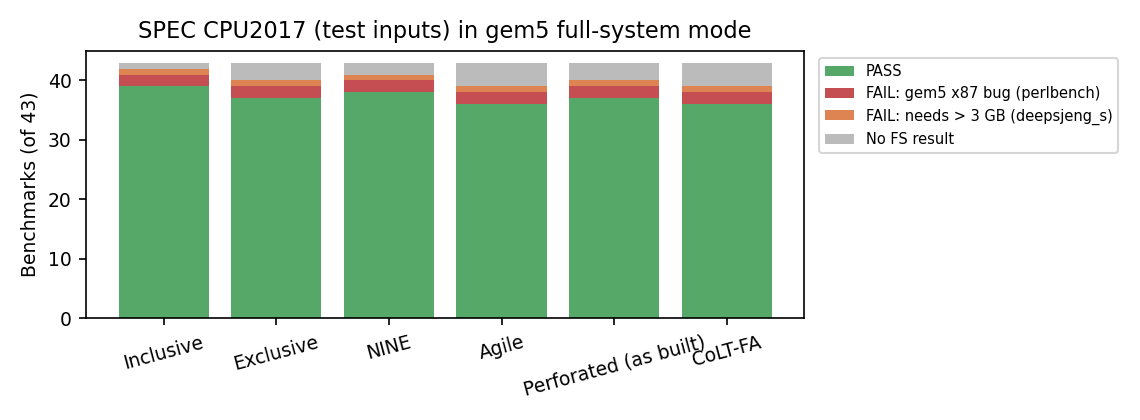
\includegraphics[width=\textwidth]{figures/spec_fs_outcome.png}
\caption{Outcome of the 43 SPEC CPU2017 benchmarks (test inputs) on each design in full-system mode.}
\label{fig:spec_outcome}
\end{figure}

\begin{table}[htbp]
\centering
\small
\caption{Full-system SPEC CPU2017 results (test inputs, out of 43).}
\label{tab:spec_outcome}
\begin{tabular}{l c c c c}
\toprule
\textbf{Design} & \textbf{PASS} & \textbf{FAIL: x87 bug} & \textbf{FAIL: memory} & \textbf{No full-system result} \\
\midrule
Inclusive & 37 & 2 & 1 & 3 \\
Exclusive & 37 & 2 & 1 & 3 \\
NINE & 37 & 2 & 1 & 3 \\
Agile / NaiveFP & 36 & 2 & 1 & 4 \\
Perforated Pages & 37 & 2 & 1 & 3 \\
CoLT-FA & 36 & 2 & 1 & 4 \\
\bottomrule
\end{tabular}
\end{table}

\begin{figure}[htbp]
\centering
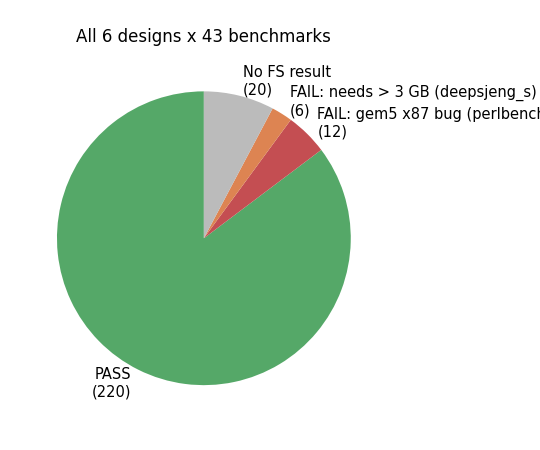
\includegraphics[width=0.45\textwidth]{figures/spec_fs_pie.png}
\caption{Outcome of all 258 benchmark runs (6 designs $\times$ 43).}
\label{fig:spec_pie}
\end{figure}

\noindent \textbf{Every benchmark that can run in this setup passes on every design.} The same three benchmarks fail on every design, and none of the failures depends on the TLB:
\begin{itemize}
    \item \textbf{500.perlbench\_r and 600.perlbench\_s} fail because of a bug in \texttt{gem5}'s emulation of x87 floating-point instructions. Perl prints long double values (\texttt{printf "\%a"}) through these instructions and the result is wrong under \texttt{gem5}. We checked that both benchmarks pass natively with the exact same SPEC setup and wrapper, and that they still fail in \texttt{gem5} with the wrapper removed. A patch to the x87 microcode was in progress at the time of writing.
    \item \textbf{631.deepsjeng\_s} needs 6.9GB of memory, more than the 3 GiB the board allows, so the program cannot start.
\end{itemize}

\noindent Four more benchmarks have no full-system pass/fail result:
\begin{itemize}
    \item \textbf{619.lbm\_s} needs 3.2GB, just above the memory limit, and \texttt{gem5} stops with an internal cache assertion when it switches back from the timing to the atomic CPU after its window. Its window statistics were saved.
    \item \textbf{525.x264\_r and 625.x264\_s} run about 1 trillion instructions each on the test input, which would take around 13 days to simulate. Their window statistics were saved.
    \item \textbf{627.cam4\_s} passes on four designs and was still running on Agile and CoLT-FA at the time of writing. It fails natively on our SPEC build but passes in \texttt{gem5}.
\end{itemize}

\subsection{The Two Large Benchmarks in SE Mode}
Since 631.deepsjeng\_s and 619.lbm\_s do not fit in the full-system guest, both were run in SE mode with 8 GiB of memory on all six designs. Each output was compared byte by byte with the native output, which had passed SPEC's check. 619.lbm\_s is an OpenMP program, so it was run with one OpenMP thread (\texttt{OMP\_NUM\_THREADS=1}).

\begin{table}[htbp]
\centering
\small
\caption{SE-mode results with 8 GiB of memory.}
\label{tab:se_bigmem}
\begin{tabular}{l c c c c c c}
\toprule
\textbf{Benchmark} & \textbf{Inclusive} & \textbf{Exclusive} & \textbf{NINE} & \textbf{Agile} & \textbf{Perforated} & \textbf{CoLT-FA} \\
\midrule
631.deepsjeng\_s & PASS & PASS & PASS & PASS & PASS & PASS \\
619.lbm\_s & PASS & PASS & PASS & PASS & PASS & PASS \\
\bottomrule
\end{tabular}
\end{table}

\noindent The CoLT-FA runs had the oracle turned on and reported 0 mismatches, with 1,600,771 buffer hits on 631.deepsjeng\_s and 62,071,327 on 619.lbm\_s.

\subsection{How Much the SPEC Test Inputs Use the TLB}
The windows also show how hard each benchmark pushes the TLB. Figure~\ref{fig:spec_pressure} plots the page walks per 1000 instructions on the Inclusive design. The highest value is 1.145 (638.imagick\_s), and benchmarks usually called memory-intensive stay low: 605.mcf\_s is 0.242, and lbm, roms and xz stay at or below about 0.5. The test inputs are small, so their working sets mostly fit in the TLB's reach. \textbf{The SPEC test-input runs are therefore mainly a correctness result}, and the performance comparison in Section~\ref{sec:perf} uses workloads that stress the TLB much more.

\begin{figure}[htbp]
\centering
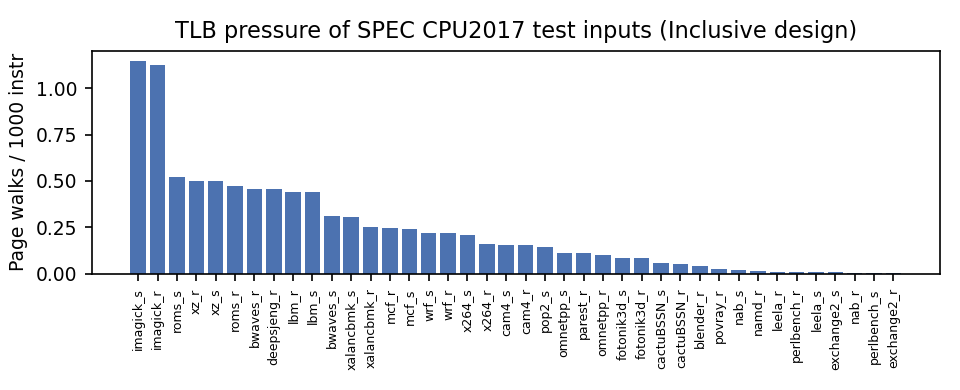
\includegraphics[width=\textwidth]{figures/spec_test_pressure.png}
\caption{Page walks per 1000 instructions for the SPEC CPU2017 test inputs (Inclusive design, 200M-instruction window).}
\label{fig:spec_pressure}
\end{figure}

% -----------------------------------------------------------------------------
\section{Performance on TLB-Intensive Workloads}
\label{sec:perf}
% -----------------------------------------------------------------------------

\subsection{Workloads}
Following the instructor's suggestion, we used the GAPBS graph benchmark suite and a key-value store, together with other standard memory-intensive programs (Table~\ref{tab:workloads}). All programs were built as static binaries and placed on a separate disk image. The GAPBS graphs were generated once in advance with GAPBS's own converter, because generating the graph took about 95\% of the instructions of a bfs run. The memcached load generator (\texttt{mc-crusher}) does not stop by itself after a fixed number of requests, so a small driver script (\texttt{run\_memcached.sh}) watches memcached's own counters and stops each phase.

\begin{table}[htbp]
\centering
\small
\caption{TLB-intensive workloads. Native data-TLB misses per 1000 instructions were measured with \texttt{perf} on a lab machine (Intel, transparent huge pages in \texttt{madvise} mode).}
\label{tab:workloads}
\begin{tabularx}{\textwidth}{l X r r}
\toprule
\textbf{Workload} & \textbf{Configuration} & \textbf{Memory} & \textbf{Native misses / 1k instr} \\
\midrule
GAPBS bfs~\cite{beamer2015gap} & Kronecker graph, $2^{20}$ vertices, 8 trials & 137MB & 0.97 \\
GAPBS pr & same graph, 10 iterations & 137MB & 0.06 \\
GAPBS cc & uniform random graph, $2^{20}$ vertices, 4 trials & 145MB & 0.26 \\
GAPBS bc & Kronecker graph, 2 trials & 151MB & 10.10 \\
GAPBS sssp & weighted Kronecker graph, 2 trials & 261MB & 3.22 \\
GAPBS tc & Kronecker graph, 1 trial & 288MB & 0.36 \\
XSBench~\cite{tramm2014xsbench} & small problem, event-based, 2M lookups & 241MB & 9.43 \\
STREAM~\cite{mccalpin1995stream} & 20M-element arrays, 3 repetitions & 480MB & 1.12 \\
memcached~\cite{memcached} & 200k keys of 1KB, then uniform random GETs with \texttt{mc-crusher} & & 0.95 \\
SPEC CPU2017 reference & mcf, omnetpp, xalancbmk, deepsjeng, xz, roms, lbm, bwaves & & \\
\bottomrule
\end{tabularx}
\end{table}

\noindent The native numbers come from a processor with a much larger second-level TLB (about 2,048 entries) than our 512-entry L2, so the same programs miss more in our simulated system.

\subsection{How the Numbers Are Compared}
The metric is \emph{page walks per 1000 instructions} in the measurement window: data-TLB misses that remain after the L1, the CoLT-FA buffer (if present) and the L2 have all missed. Lower is better. Two rules were followed for every comparison, because of what the data showed:
\begin{itemize}
    \item \textbf{With transparent huge pages off}, results are stable across machines. For example, bfs gave 1.219 to 1.253 walks per 1000 instructions for the four non-CoLT designs, which ran on three different machines, so these runs are compared across machines.
    \item \textbf{With transparent huge pages on}, results depend on the machine. Each machine built its own disk image, and how the guest places huge pages in memory changed with it. The same NINE configuration gave 2.16 walks per 1000 instructions for bc on one machine and 6.04 on another, while repeating a run on the \emph{same} machine gave exactly the same statistics. Huge-pages-on results are therefore only compared between runs on the same machine.
\end{itemize}

\subsection{All Designs With Huge Pages Off}
Figure~\ref{fig:thpoff_all} and Table~\ref{tab:thpoff_all} compare all designs with transparent huge pages turned off in the guest, so every page is 4KB.

\begin{figure}[htbp]
\centering
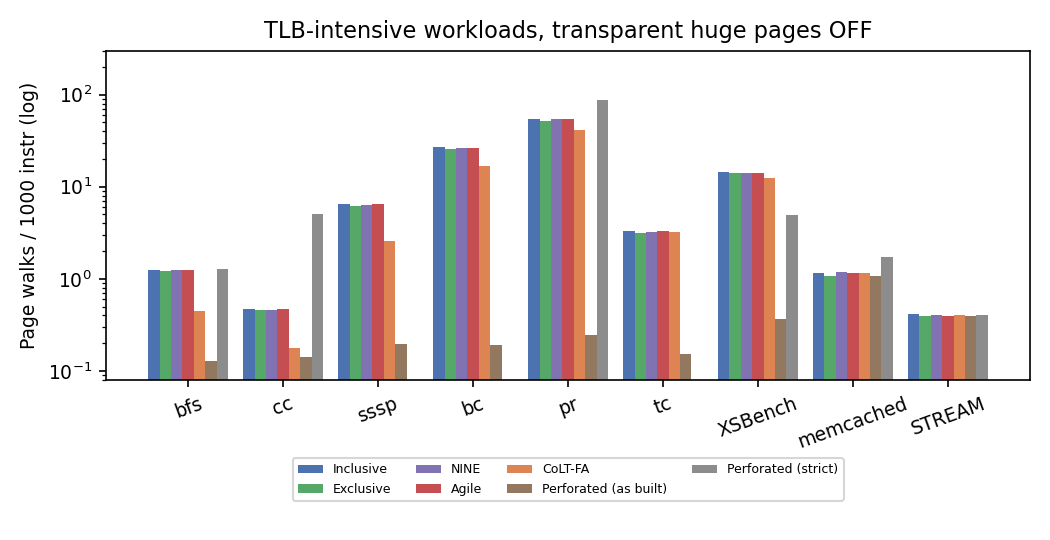
\includegraphics[width=\textwidth]{figures/thp_off_all_designs.png}
\caption{Page walks per 1000 instructions with transparent huge pages off (log scale).}
\label{fig:thpoff_all}
\end{figure}

\begin{table}[htbp]
\centering
\small
\caption{Page walks per 1000 instructions, transparent huge pages off. "Perf." is Perforated Pages as built and "Strict" is the strict variant from Section~\ref{sec:perf_strict}; a dash means not run.}
\label{tab:thpoff_all}
\begin{tabular}{l r r r r r r r}
\toprule
\textbf{Workload} & \textbf{Inclusive} & \textbf{Exclusive} & \textbf{NINE} & \textbf{Agile} & \textbf{CoLT-FA} & \textbf{Perf.} & \textbf{Strict} \\
\midrule
GAPBS bfs & 1.253 & 1.219 & 1.234 & 1.236 & 0.448 & 0.129 & 1.290 \\
GAPBS cc & 0.471 & 0.463 & 0.461 & 0.464 & 0.178 & 0.140 & 5.056 \\
GAPBS sssp & 6.461 & 6.251 & 6.353 & 6.435 & 2.585 & 0.197 & -- \\
GAPBS bc & 26.743 & 25.848 & 26.551 & 26.646 & 16.911 & 0.192 & -- \\
GAPBS pr & 55.046 & 51.821 & 54.760 & 54.692 & 41.812 & 0.244 & 88.556 \\
GAPBS tc & 3.279 & 3.142 & 3.249 & 3.266 & 3.220 & 0.154 & -- \\
XSBench & 14.395 & 13.967 & 14.256 & 14.254 & 12.492 & 0.369 & 4.941 \\
memcached & 1.156 & 1.082 & 1.178 & 1.156 & 1.142 & 1.081 & 1.728 \\
STREAM & 0.414 & 0.399 & 0.400 & 0.399 & 0.400 & 0.399 & 0.400 \\
\bottomrule
\end{tabular}
\end{table}

\noindent Among the inclusion policies, Exclusive gives the fewest walks on every workload (STREAM is a tie), because it does not keep the same translation in both levels and so holds more translations in total (for pr, 51.821 against 55.046 for Inclusive, about 6\% fewer). Inclusive gives the most. The Agile prefetcher gives almost the same numbers as NINE on these workloads. CoLT-FA gives the largest reduction of the realistic designs. Perforated Pages as built shows very low numbers; Section~\ref{sec:perf_strict} explains why these numbers are not realistic.

\subsection{CoLT-FA Compared With NINE}
CoLT-FA is built on NINE, and the same binary runs both. Figure~\ref{fig:colt_vs_nine} shows the change in page walks with huge pages off.

\begin{figure}[htbp]
\centering
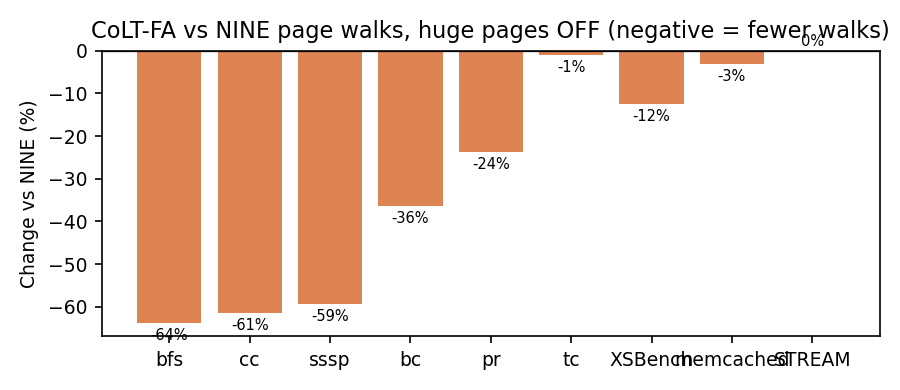
\includegraphics[width=0.85\textwidth]{figures/colt_vs_nine_thpoff.png}
\caption{Change in page walks of CoLT-FA (8 entries) compared with NINE, transparent huge pages off.}
\label{fig:colt_vs_nine}
\end{figure}

\begin{table}[htbp]
\centering
\small
\caption{CoLT-FA (8 entries) against NINE, transparent huge pages off (page walks per 1000 instructions).}
\label{tab:colt_vs_nine}
\begin{tabular}{l r r r}
\toprule
\textbf{Workload} & \textbf{NINE} & \textbf{CoLT-FA} & \textbf{Change} \\
\midrule
GAPBS bfs & 1.234 & 0.448 & $-63.7\%$ \\
GAPBS cc & 0.461 & 0.178 & $-61.4\%$ \\
GAPBS sssp & 6.353 & 2.585 & $-59.3\%$ \\
GAPBS bc & 26.551 & 16.911 & $-36.3\%$ \\
GAPBS pr & 54.760 & 41.812 & $-23.6\%$ \\
XSBench & 14.256 & 12.492 & $-12.4\%$ \\
memcached & 1.178 & 1.142 & $-3.1\%$ \\
GAPBS tc & 3.249 & 3.220 & $-0.9\%$ \\
STREAM & 0.400 & 0.400 & $0.0\%$ \\
\bottomrule
\end{tabular}
\end{table}

\noindent CoLT-FA reduces page walks most on the graph kernels bfs, cc and sssp, by about 59\% to 64\%, and by 36\% and 24\% on bc and pr. These kernels read the graph's large arrays, which the operating system often places on physically contiguous 4KB pages, and that is exactly what CoLT can merge. On XSBench the reduction is 12\%. On memcached, tc and STREAM it is small or zero. For STREAM the buffer received very few hits (57 with 8 entries), which means that in this run the guest did not give STREAM's arrays physically contiguous pages, and CoLT can only merge contiguous pages.

\paragraph{Buffer size.} Figure~\ref{fig:colt_size} compares the default 8-entry buffer with a 32-entry buffer. Going from 8 to 32 entries reduces walks a little further on some workloads (pr from 41.812 to 38.420, bfs from 0.448 to 0.424), but most of the benefit already comes with 8 entries.

\begin{figure}[htbp]
\centering
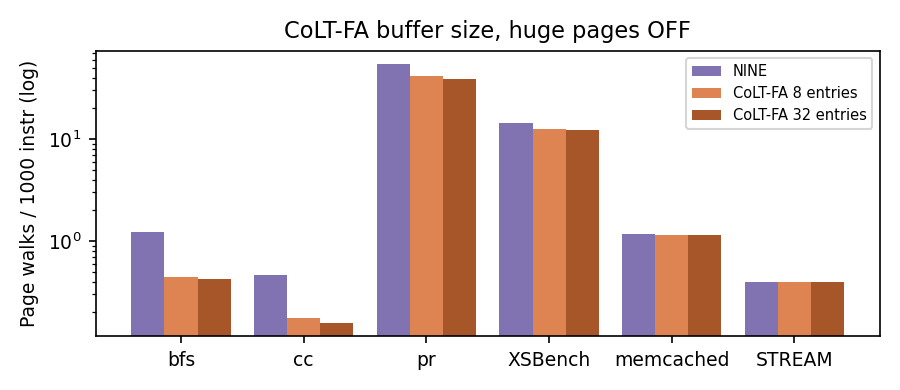
\includegraphics[width=0.85\textwidth]{figures/colt_size.png}
\caption{NINE, CoLT-FA with 8 entries and CoLT-FA with 32 entries, transparent huge pages off.}
\label{fig:colt_size}
\end{figure}

\paragraph{With huge pages on.} Following the same-machine rule, the comparison with huge pages on uses NINE and CoLT-FA runs from the same machine (Table~\ref{tab:colt_thpon} and Figure~\ref{fig:colt_thpon}).

\begin{table}[htbp]
\centering
\small
\caption{CoLT-FA (8 entries) against NINE with transparent huge pages on, each pair from the same machine (page walks per 1000 instructions).}
\label{tab:colt_thpon}
\begin{tabular}{l l r r r}
\toprule
\textbf{Workload} & \textbf{Machine} & \textbf{NINE} & \textbf{CoLT-FA} & \textbf{Change} \\
\midrule
GAPBS bfs & csews36 & 0.118 & 0.062 & $-47.5\%$ \\
GAPBS pr & csews36 & 2.687 & 1.914 & $-28.8\%$ \\
GAPBS bc & csews30 & 6.038 & 4.309 & $-28.6\%$ \\
GAPBS sssp & csews30 & 3.619 & 2.742 & $-24.2\%$ \\
GAPBS cc & csews36 & 0.028 & 0.024 & $-14.3\%$ \\
XSBench & csews36 & 1.138 & 1.102 & $-3.2\%$ \\
STREAM & csews36 & 0.012 & 0.010 & $-16.7\%$ \\
\midrule
519.lbm\_r (ref) & csews24 & 0.375 & 0.076 & $-79.7\%$ \\
523.xalancbmk\_r (ref) & csews24 & 2.608 & 1.453 & $-44.3\%$ \\
520.omnetpp\_r (ref) & csews24 & 2.226 & 1.751 & $-21.3\%$ \\
505.mcf\_r (ref) & csews24 & 3.655 & 3.614 & $-1.1\%$ \\
\bottomrule
\end{tabular}
\end{table}

\noindent With huge pages on, CoLT-FA still reduces page walks, by 47.5\% on bfs and by about 24\% to 29\% on pr, bc and sssp. The absolute numbers are much smaller than with huge pages off, so the remaining walks come from memory that is still mapped with 4KB pages, which is the part CoLT-FA can coalesce. On cc and STREAM the values are very small (below 0.03), so their percentages rest on few walks. The four SPEC reference benchmarks in the lower part of the table were also run on one machine with the same binary. CoLT-FA reduces walks by 79.7\% on lbm, 44.3\% on xalancbmk and 21.3\% on omnetpp, while mcf is almost unchanged ($-1.1\%$).

\begin{figure}[htbp]
\centering
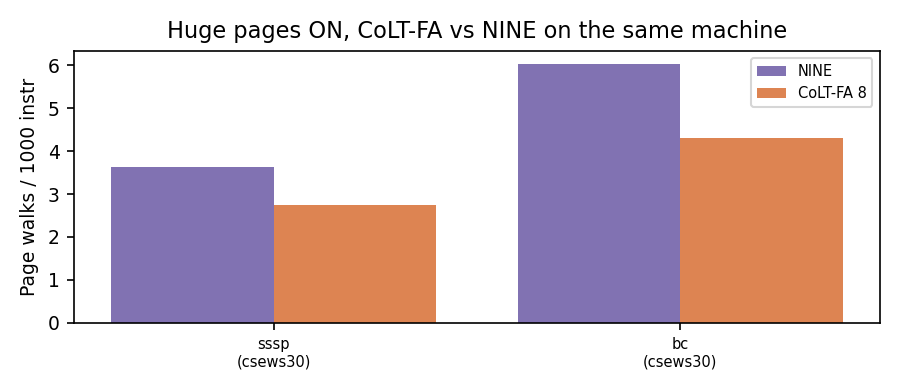
\includegraphics[width=0.75\textwidth]{figures/colt_vs_nine_thpon_samehost.png}
\caption{CoLT-FA against NINE with transparent huge pages on, both runs on the same machine.}
\label{fig:colt_thpon}
\end{figure}

\subsection{The Effect of Huge Pages}
Figure~\ref{fig:thp_effect} shows NINE with transparent huge pages off and on, from the same binary on the same machine. Huge pages remove most of the page walks: pr goes from 54.760 to 2.687, XSBench from 14.256 to 1.138, and bfs from 1.234 to 0.118. memcached barely changes (1.178 to 1.117). This shows that, when the operating system can give a program 2MB pages, much of the TLB pressure disappears, and the designs then differ less. CoLT-FA is most useful in the opposite case, when memory ends up in 4KB pages.

\begin{figure}[htbp]
\centering
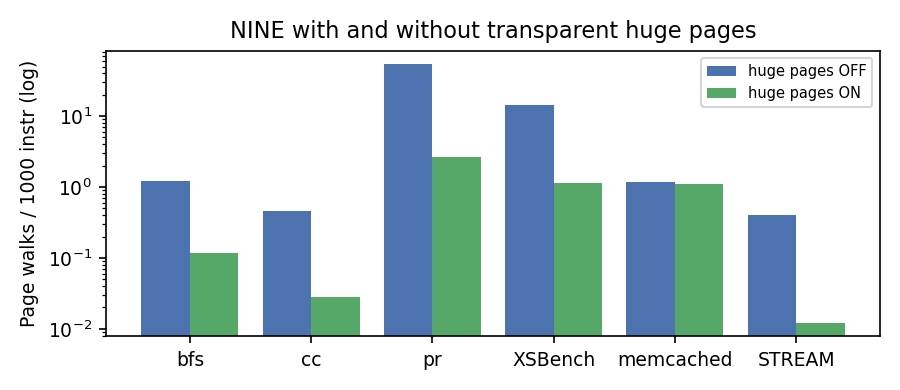
\includegraphics[width=0.85\textwidth]{figures/thp_effect_nine.png}
\caption{NINE with transparent huge pages off and on (same binary, same machine).}
\label{fig:thp_effect}
\end{figure}

\subsection{SPEC CPU2017 Reference Inputs}
Nine SPEC benchmarks were run with reference inputs, measured for 200M instructions after 3G instructions of warm-up, with huge pages on. Each design ran on its own machine, so following the rule above these numbers are reported per design and are not used for small differences. Table~\ref{tab:ref} shows the results for the four inclusion and prefetching designs, which agree with each other closely. With real input sizes mcf (3.360 to 3.695) and omnetpp (2.172 to 2.324) are the most TLB-intensive, far above their test-input values.

\begin{table}[htbp]
\centering
\small
\caption{SPEC CPU2017 reference inputs, page walks per 1000 instructions (huge pages on, each design on its own machine).}
\label{tab:ref}
\begin{tabular}{l r r r r}
\toprule
\textbf{Benchmark} & \textbf{Inclusive} & \textbf{Exclusive} & \textbf{NINE} & \textbf{Agile} \\
\midrule
505.mcf\_r & 3.695 & 3.360 & 3.617 & 3.613 \\
523.xalancbmk\_r & 2.625 & 2.623 & 2.609 & 2.614 \\
520.omnetpp\_r & 2.324 & 2.172 & 2.232 & 2.267 \\
503.bwaves\_r & 0.486 & 0.476 & 0.481 & 0.483 \\
519.lbm\_r & 0.378 & 0.369 & 0.374 & 0.375 \\
554.roms\_r & 0.346 & 0.333 & 0.340 & 0.344 \\
531.deepsjeng\_r & 0.171 & 0.161 & 0.164 & 0.165 \\
557.xz\_r & 0.132 & 0.128 & 0.129 & 0.133 \\
\bottomrule
\end{tabular}
\end{table}

\noindent 549.fotonik3d\_r gave no window on any design: its first program finished before the 3G-instruction warm-up ended.

% -----------------------------------------------------------------------------
\section{A Second Look at Perforated Pages}
\label{sec:perf_strict}
% -----------------------------------------------------------------------------

In Table~\ref{tab:thpoff_all}, Perforated Pages as built shows close to zero page walks on almost every workload, far fewer than any other design. While looking into this we found the reason in the model itself. Each L2 entry covers a 2MB virtual region, but it stores a \emph{separate physical address for each of its 512 4KB pages} (\texttt{paddrs[512]}), and it never checks that these pages are physically contiguous. With 128 sets of 4 ways, the L2 can therefore hold up to $128 \times 4 \times 512 = 262{,}144$ unrelated 4KB translations, about 512 times the reach of the other designs' 512-entry L2. Real perforated pages are 2MB regions that are physically contiguous apart from their holes, so one base address and a bitmap are enough to describe them.

To measure the design under the paper's rule, we added a strict mode (\texttt{PERF\_STRICT=1}, produced by \texttt{robustness/patches/make\_perf\_strict.py}). A 4KB page may join a region only if its physical address equals the region's base address plus its offset. Otherwise the region is started again from the new page. The default behaviour is unchanged, so the earlier results stay reproducible.

\begin{table}[htbp]
\centering
\small
\caption{Perforated Pages as built and in strict mode, compared with NINE (page walks per 1000 instructions).}
\label{tab:perf_strict}
\begin{tabular}{l l r r r}
\toprule
\textbf{Workload} & \textbf{Huge pages} & \textbf{NINE} & \textbf{As built} & \textbf{Strict} \\
\midrule
GAPBS bfs & off & 1.234 & 0.129 & 1.290 \\
GAPBS cc & off & 0.461 & 0.140 & 5.056 \\
GAPBS pr & off & 54.760 & 0.244 & 88.556 \\
XSBench & off & 14.256 & 0.369 & 4.941 \\
memcached & off & 1.178 & 1.081 & 1.728 \\
505.mcf\_r (ref) & on & 3.617 & 0.124 & 10.352 \\
520.omnetpp\_r (ref) & on & 2.232 & 0.567 & 9.058 \\
523.xalancbmk\_r (ref) & on & 2.609 & 0.185 & 4.899 \\
\bottomrule
\end{tabular}
\end{table}

\noindent With the strict rule, Perforated Pages has \emph{more} page walks than NINE on most workloads (for example pr 88.556 against 54.760, and mcf 10.352 against 3.617). Every entry is tied to a 2MB virtual region, so memory made of scattered 4KB pages wastes most of each entry, and regions are restarted often. XSBench is the exception (4.941 against 14.256). We conclude that the large gains measured for Perforated Pages in this project, including those in Section~6 of Part~\ref{part:mid}, come mostly from the unlimited per-page storage of the model and not from the perforated-page idea. A fair evaluation of Perforated Pages would also need the operating system support from the paper, which creates the sparse 2MB regions in the first place. For these reasons we treat CoLT-FA as the main realistic design of this project.

% -----------------------------------------------------------------------------
\section{Limitations and Notes on Method}
\label{sec:limits}
% -----------------------------------------------------------------------------
\begin{itemize}
    \item \textbf{Memory limit.} The \texttt{X86Board} allows at most 3 GiB of guest memory, so 631.deepsjeng\_s and 619.lbm\_s were checked in SE mode only (both PASS on all designs).
    \item \textbf{x87 emulation.} The perlbench failures are caused by \texttt{gem5}, not by the TLB designs, and affect every design.
    \item \textbf{Sampled windows.} Performance numbers come from windows of 200M to 1.5G instructions, not from whole runs. Correctness is still checked over the whole run for SPEC test inputs.
    \item \textbf{Same-machine rule.} With transparent huge pages on, the guest's memory layout depends on the disk image built on each machine, so these results are only compared within one machine.
    \item \textbf{Single core.} All full-system runs use one simulated core.
    \item \textbf{Redis.} Redis was also prepared as a second key-value store. The first runs stopped making progress inside the guest before the measured phase and were stopped after two days. A second attempt with time limits and progress messages on every step was started on the last day. memcached covers the key-value store case in this report.
    \item \textbf{The Hybrid L2 TLB} from Part~\ref{part:mid} was not part of the second phase.
\end{itemize}

% -----------------------------------------------------------------------------
\section{Conclusion}
% -----------------------------------------------------------------------------
In the first half of the project we built set-associative L2 TLB designs with different inclusion policies, prefetching, CoLT-FA, Perforated Pages and a Hybrid in \texttt{gem5}, and measured them in SE mode on microbenchmarks. In the second half we audited all of them and fixed the problems that only show up under a real operating system: missing L2 invalidation on unmaps and address-space switches, PCID handling, checkpointing, and hard-coded permissions. We added a translation oracle and invariant checkers and found no translation error in any design. We rebuilt CoLT-FA so that it coalesces pages from the hardware page walker, as in the original paper, which made it work in full-system mode for the first time.

In full-system mode on an Ubuntu guest, every SPEC CPU2017 benchmark that the simulator can run passed on all six designs. The only failures came from a \texttt{gem5} floating-point emulation bug and from the 3 GiB memory limit, and the two large benchmarks passed in SE mode with more memory. On the graph and key-value workloads, CoLT-FA reduced page walks compared with NINE by 59\% to 64\% on bfs, cc and sssp, by 36\% on bc and by 24\% on pr with 4KB pages, and, on the same machine with huge pages on, by 47.5\% on bfs and by about 24\% to 29\% on pr, bc and sssp. On SPEC reference inputs it reduced walks by 79.7\% on lbm, 44.3\% on xalancbmk and 21.3\% on omnetpp. Exclusive was the best of the inclusion policies. A closer look at Perforated Pages showed that its large gains came from an unrealistic model, and under the paper's rule it did worse than NINE on most workloads.
